\documentclass[12pt]{article}
\usepackage{geometry}
\usepackage{graphicx} % 插图
\usepackage{float} % 插图位置固定
\usepackage{amsmath} % 文字加粗
\usepackage[UTF8]{ctex} %中文宏包
\setCJKmainfont{SimSun}
\usepackage{fontspec} %引入字体设置宏包
\setmainfont{Times New Roman}
\usepackage{indentfirst} %首行缩进
\usepackage{listings} %代码
\usepackage{color} %字体颜色
\usepackage{subfigure}  %插入多图时用子图显示的宏包

\usepackage{minted} %代码
\usemintedstyle{vs}


%\usepackage{fancyhdr} %页眉页脚
%\pagestyle{fancy} 
%\fancyhf{}
%\lhead{数字图像处理}
%\chead{Noise Reduction Using a Median Filter}
%\rhead{张青铭 \quad 3200105426}
%\renewcommand{\headrulewidth}{0pt}
%图片路径
\graphicspath{ {figures/} }

%页面格式
\geometry{a4paper,
	left=20mm,
	right=20mm,
	top=20mm,
	bottom=20mm }

\title{{\Huge{\textbf{数字图像处理}}}\\Pro6-2\quad  Pseudo-Color Image Processing}
\author{信息与电子工程学院\quad 信息工程 \quad 3200105426\\张青铭}
\date{\today}

\begin{document}
\maketitle
\section{实验任务}
(1)实现图6.23,可以为输入图像指定两个灰度值范围,并输出RGB图像,该图像的像素是具有与输入图像中的一个灰度范围相对应的指定颜色,并且RGB图像中的其余像素具有与输入图像中相同的灰度。可以将输入颜色限制为图6.4(a)中的所有颜色。

(2)对图1.10(4)用程序进行处理,使河流呈现黄色,其余像素与输入图像中的灰度相同。
\section{算法设计}
1.灰度分层:

对于最简单的对于一张灰度图像,每一个像素点都对应一个灰度值。我们在灰度轴设置一个阈值,低于该阈值的像素点对应一种颜色,高于该阈值对应另一种颜色(理解为将图像二值化)。本实现设置灰度域:0,63、64,127、128,191、192,255四个范围,分别输出蓝色、紫色、黄色、红色。对于任务二,设定将灰度值为0的部分替代为黄色,只设置0与大于0两个通道。
\\

2.灰度到彩色的变换:

彩色图像由三个通道(RGB),而灰度图像只有一个通道。对于灰度图像,可以将灰度值执行三个独立的变换,将变换的结果作为三个通道合成一张彩色图片。变换函数可以根据特定的情况进行调制。上一节的灰度分层身成为彩色图像使用的是分段线性函数。而这种变换是以平滑的非线性函数为基础的。程序原理图如下:
\\

3.融合三通道结果,输出最终图像
\begin{figure}[H]
	\centering
	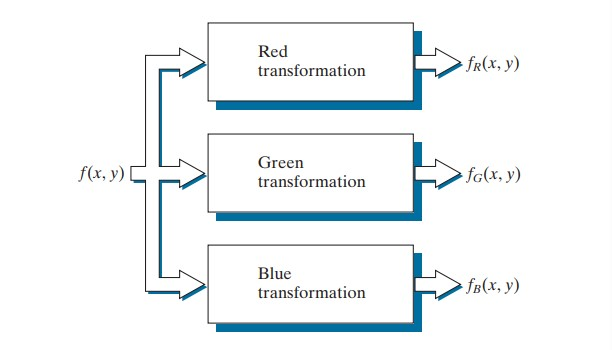
\includegraphics[width=0.5\linewidth]{figures/1}
	\caption{RBG三通道变换}
\end{figure}

\section{代码实现}
\begin{minted}[frame=lines,tabsize=4,python3,baselinestretch=0.85]{matlab}
close all;clc;clear;
%% first task
% load image and display
img = imread('Fig623.tif');
figure(1);subplot(1,2,1);
imshow(img);
title('original image');

% read basic image information
img = double(img);
[M, N] = size(img);
gray_level = 256;
R = zeros(M, N);
G = zeros(M, N);
B = zeros(M, N);

% process four gray levels separately
for i = 1:M
	for j = 1:N
		if(img(i, j) < gray_level/4)
			R(i, j) = 0;
			G(i, j) = 4 * img(i, j);
			B(i, j) = gray_level;
		else if(img(i, j) < gray_level/2)
			R(i, j) = 0;
			G(i, j) = gray_level;
			B(i, j) = gray_level*2 - 4 * img(i, j);
			else if(img(i, j) < 3*gray_level/4)
				R(i, j) = 4 * img(i, j) - gray_level*2;
				G(i, j) = gray_level;
				B(i, j) = 0;
				else
					R(i, j) = gray_level;
					G(i, j) = 4 * gray_level - 4 * img(i, j);
					B(i, j) = 0;
				end
			end
		end
	end
end

% merge three channels of RBG
img1 = zeros(M, N);
for i = 1:M
	for j = 1:N
		img1(i, j, 1) = R(i, j);
		img1(i, j, 2) = G(i, j);
		img1(i, j, 3) = B(i, j);
	end
end
img1 = img1 / 256;

subplot(1,2,2);
imshow(img1);
title('Pseudo-Color');
%% second task
close all;clc;clear;

% load image and display
img = imread('Fig110.tif');
figure(1);subplot(1,2,1);
imshow(img);
title('original image');

% read basic image information
img = double(img);
[M, N] = size(img);
gray_level = 256;
R = zeros(M, N);
G = zeros(M, N);
B = zeros(M, N);

% process four gray levels separately
for i = 1:M
	for j = 1:N
		if(img(i, j) < 20)
			R(i,j) = gray_level;
			G(i,j) = gray_level;
			B(i,j) = 0;
		else if(img(i, j) > 1)
			R(i, j) = img(i, j);
			G(i, j) = img(i, j);
			B(i, j) = img(i, j);
			end
		end
	end
end

% merge three channels of RBG
img1 = zeros(M, N);
for i = 1:M
	for j = 1:N
		img1(i, j, 1) = R(i, j);
		img1(i, j, 2) = G(i, j);
		img1(i, j, 3) = B(i, j);
	end
end
img1 = img1 / 256;

subplot(1,2,2);
imshow(img1);
title('Pseudo-Color');
\end{minted}

\section{实验结果}
图6.23处理结果如下,可以发现基本灰度值最小的部分颜色为蓝色、灰度值最大的部分颜色为红色,中间部分为黄色和绿色,符合预期结果,也符合程序代码。
\begin{figure}[H]
	\centering
	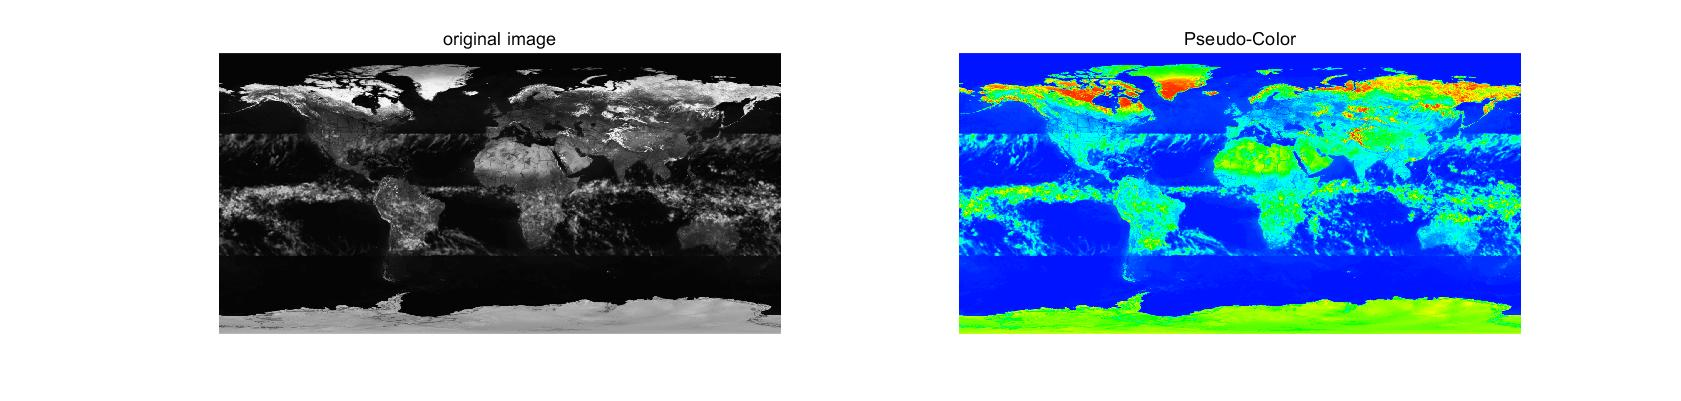
\includegraphics[width=1\linewidth]{figures/2}
	\caption{伪彩色处理}
\end{figure}

图1.10处理结果如下,从结果图对比可以看出,基本能够分离出河流部分并将其赋为黄色。
\begin{figure}[H]
	\centering
	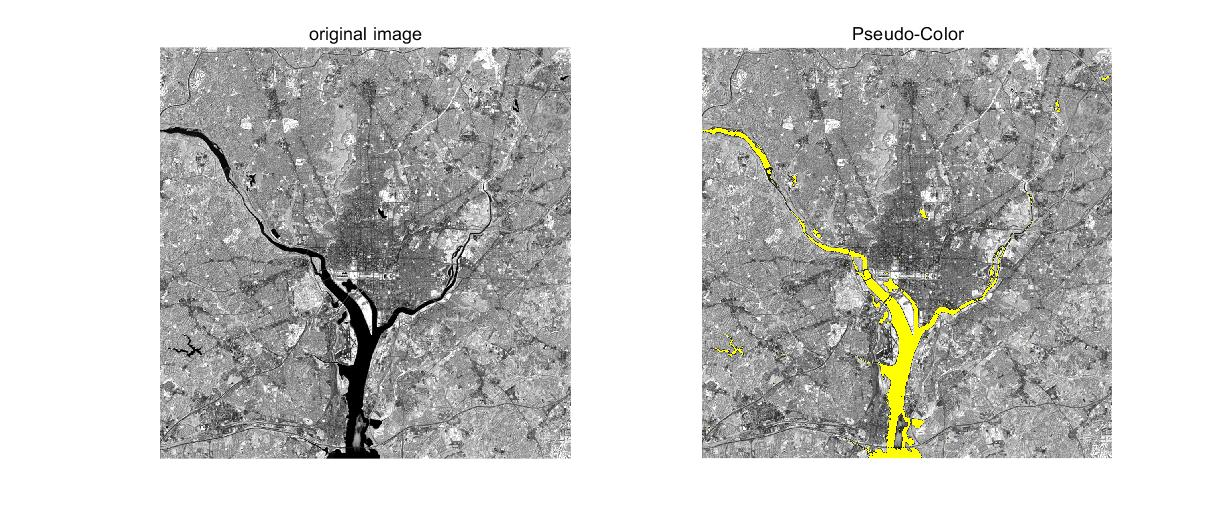
\includegraphics[width=0.8\linewidth]{figures/3}
	\caption{河流赋黄色}
\end{figure}
\section{总结}
本次实验完成了灰度图像的伪彩色处理。通过这次实验我对于色彩RGB的融合有了更深的理解,并且从本质上RGB三通道由灰度图像构建了彩色图像。这个过程十分有成就感,非常直接。

这次实验的关键在于灰度集的分层,以及颜色的赋值处理,我根据了教材上图6.4的混合颜色标准完成了指定颜色的赋值。其余代码部分都比较简单基础,综合来说对于理论知识的帮助比较大。

\end{document}
